\documentclass[tikz,border=8pt]{standalone}
\usetikzlibrary{arrows.meta,positioning,fit}
\begin{document}
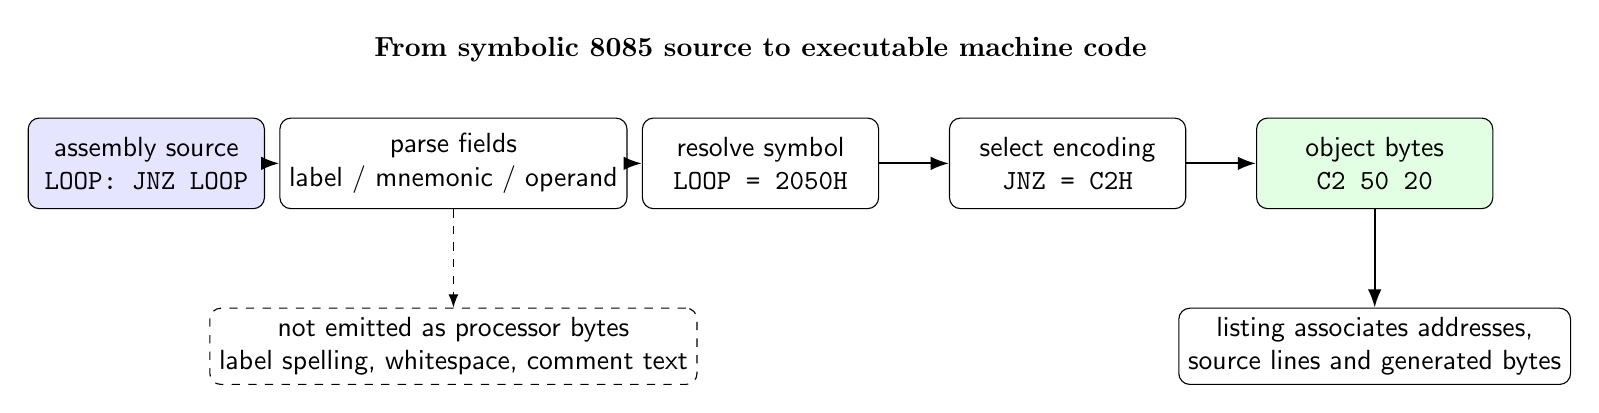
\begin{tikzpicture}[
  font=\sffamily,
  >=Latex,
  block/.style={draw,rounded corners,minimum width=3.0cm,minimum height=1.15cm,align=center},
  flow/.style={->,thick}
]
\node[block,fill=blue!10] (src) at (0,0) {assembly source\\\texttt{LOOP: JNZ LOOP}};
\node[block] (parse) at (3.9,0) {parse fields\\label / mnemonic / operand};
\node[block] (sym) at (7.8,0) {resolve symbol\\\texttt{LOOP = 2050H}};
\node[block] (enc) at (11.7,0) {select encoding\\\texttt{JNZ = C2H}};
\node[block,fill=green!11] (obj) at (15.6,0) {object bytes\\\texttt{C2 50 20}};

\draw[flow] (src) -- (parse);
\draw[flow] (parse) -- (sym);
\draw[flow] (sym) -- (enc);
\draw[flow] (enc) -- (obj);

\node[draw,dashed,rounded corners,below=1.25cm of parse,align=center,minimum width=4.2cm] (notemit)
  {not emitted as processor bytes\\label spelling, whitespace, comment text};
\draw[->,dashed] (parse) -- (notemit);
\node[draw,rounded corners,below=1.25cm of obj,align=center,minimum width=3.8cm] (listing)
  {listing associates addresses,\\source lines and generated bytes};
\draw[flow] (obj) -- (listing);

\node[font=\bfseries] at (7.8,1.45) {From symbolic 8085 source to executable machine code};
\end{tikzpicture}
\end{document}
